\clearpage
\subsection{Jumping} % (fold)
\label{sub:jump}

The jump statements allow you to alter the sequence of instructions in the code, getting the computer to jump to another instruction.

\begin{figure}[h]
   \centering
   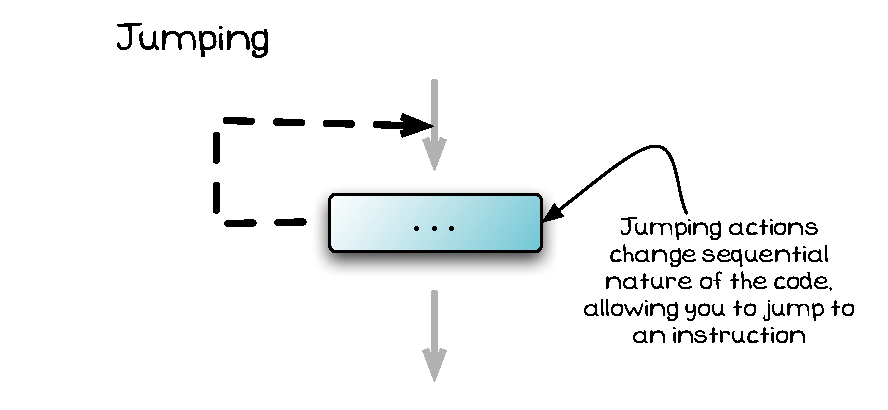
\includegraphics[width=\textwidth]{./topics/control-flow/diagrams/JumpStatements} 
   \caption{Jump Statements cause control to jump to another location in the code}
   \label{fig:looping-jump-statements}
\end{figure}

\mynote{
\begin{itemize}
  \item The jump statements are \textbf{actions}, they allow you to alter the standard sequence of the instructions and have the computer jump to a another location in the instructions.
  \item \textbf{Structured Programming} was proposed as a means of providing order and structure to the control flow through the code. These jump statements complicate this sequential flow, but in some cases they are able to simplify code.
  \item Structured jump statements allow you to control the sequence of actions related to a \nameref{sub:looping} statement, a \nameref{sub:function}, or a \nameref{sub:procedure}. These work the looping and procedural structures used in structured programming.
  \item Unstructured jump statements allow you to jump to any instruction within the code. You need to be aware that these statements exist, but they should not be used.
\end{itemize}
}

% subsection jump_statements (end)